\chapter{Background}

Feature and classifier selection are both crucial for classification using machine learning; analyzing the key properties of a dataset with the model best suited for that domain tends to lead to better results.  Classical machine learning classifiers require numerical values to represent observations of each class.  Since the datasets in natural language processing (NLP) tasks are usually raw text, as is the case for this research study, there must be a conscientious choice on how to accurately portray the text numerically.  Two NLP techniques to produce vectorized representations of text documents are presented in this chapter: term frequency-inverse document frequency score weighting, and word embeddings.  This chapter also includes a section on preprocessing techniques to refine the textual data, as well as a brief synopsis on the field of sentiment analysis to motivate the idea that sentiment scores can be important features for this study since they provide insight about the motivation and purpose of a piece of text.  Lastly, this chapter formally introduces the classifier models used in this research: k-nearest neighbors, support vector machines, and recurrent neural networks.


\section{Preprocessing} \label{preprocessingSection}
Real-world data is usually messy.  One of the first steps before performing any data analysis is to clean or refine the data by making the data structured and correct, and removing any discernible noise.  The preprocessing steps performed in this study fall into the category Jurafsky and Martin call "text normalization" because the text is being converted into a convenient and standard form \cite{preprocessing}.  The very first step in text processing is to tokenize the data, or separate the words.  Though common practice is to simply use whitespace and punctuation to delimit words, compound words such as proper nouns (e.g., "White House") can lose their meaning when broken up.  To overcome this information loss, named entity recognizers can be used to prevent splitting up these tokens.

To standardize the data, the tokens may then be converted to their roots so different tenses of words can be linked together.  However, this task, called lemmatization, requires that the words in each sentence are first tagged with their part-of-speech to determine the root word.  Since part-of-speech tagging is sometimes too computationally intensive for large documents, a simpler approach called stemming is often used in its place.  Stemming aims to remove the suffixes of each word to get the root.  However, the effectiveness of the stemmer is implementation dependent.  For example, the Porter stemmer aims to remove suffixes using pattern matching, potentially producing incoherent words or semantically incorrect words (e.g., the stem of "ties" is "ti", and the stem of "operator" is "operate") \cite{porterStemmer}.  Finally, to refine the text of the document, articles, pronouns, prepositions, and other uninformative words are sometimes filtered out before the core analysis is performed.  These uninformative words, called stop words, usually help in information retrieval and document similarity tasks \cite{stopWord}.


\section{Term Frequency-Inverse Document Frequency} \label{tfidfSection}

Once preprocessing is complete, the remaining text must be transformed into real-valued vectors so that the text can be used by a model.  One technique to produce numerical values for words in a document is to represent each word by its term frequency-inverse document frequency score.  The term frequency-inverse document frequency (tf-idf) of a word is used to quantify the importance of a word in a corpus based on how frequently the word shows up in a document and how many other documents also contain the word \cite{tfidf}.

\begin{equation}
\label{eq:tfidf}
\mbox{tf-idf}_{w,d_{i},D} = ( \frac{c_{w}}{|d_{i}|} ) \cdot \log ( \frac{|D|}{1 + |d  \in  D : w  \in  d|} ) 
\end{equation}

A basic tf-idf scoring function is available in Eq. \ref{eq:tfidf}.  The first term represents the term frequency (tf) of the word $w$, which is the ratio of the number of occurrences of the word ($c_{w}$) to the total number of words in the document ($|d_{i}|$).  The second term is the inverse document frequency (idf) which serves to boost rarer, more informative words, and diminish the impact of frequently used non-informative words, like articles and pronouns.  Since the idf is computed by taking the logarithm of the total number of documents in the corpus ($|D|$) divided by the number of documents with the word offset by 1 to avoid 0 denominators ($1 + |d  \in  D : w  \in  d|$), words that appear in almost all the documents will have a idf close to 0.  On the other hand, words that appear in only select documents will have larger idf values, thereby increasing their tf-idf weights.

\section{Word Embeddings}

\begin{figure}[h]
\centering
\captionsetup{justification=centering,width=0.95\textwidth}
\centerline{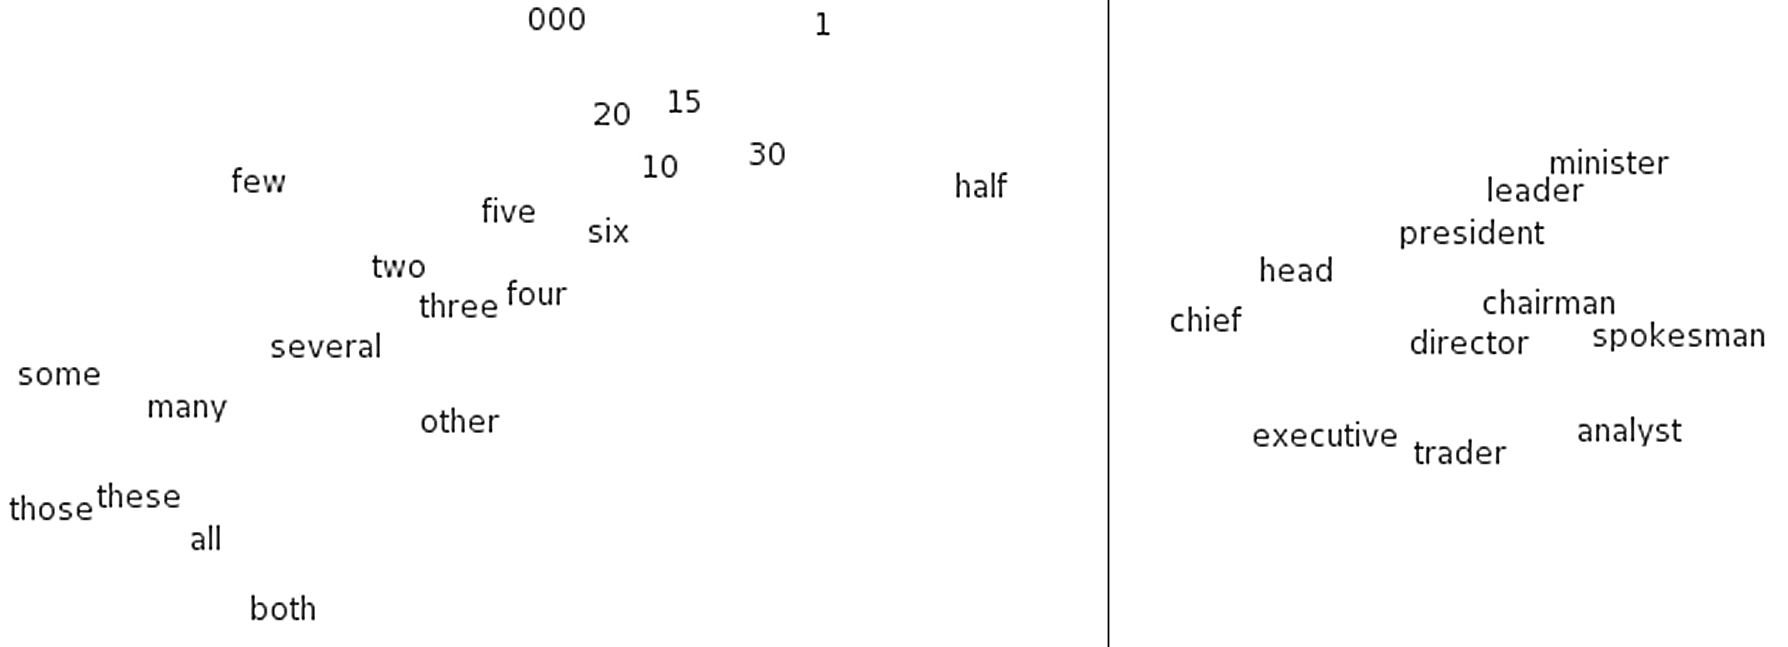
\includegraphics[width=0.95\textwidth]{similarWordVectors.png}}
\caption[t-SNE Visual of Numbers and Occupations]{
    t-SNE visualization of word embeddings \cite{wordEmbeddingImg}\\
    Left: the number region in a word embedding model\\
    Right: the occupations region
}
\label{fig:similarWordVectors}
\end{figure}


Another way to numerically represent a text is to use a word embedding model to transform each word into a real-valued vector.  The word embedding of a word is the high-dimensional vector that is the result of mapping the word with a parameterized function that was developed using a large corpus that is representative of the source language.  One of the primary benefits of using word embeddings is that similar words will tend to map to the same region.  t-distributed stochastic neighbor embedding (t-SNE) is a probabilistic technique designed for dimensionality reduction, and can be used to visualize high-dimensional datasets like word embeddings \cite{tsneAbout}.  The t-SNE algorithm converts similarities between data points into joint probabilities and tries to minimize the divergence between these joint probabilities and the high-dimensional data \cite{tsneVisual, tsnePython}.  Due to the reduction in dimensionality, mainly for the purposes of visualization, the axes and its units on t-SNE plots do not have any real meaning; however, the t-SNE still meaningfully shows which of the points are closer together in the original feature space \cite{tsneAxes}.  An example of the benefit is shown in Fig. \ref{fig:similarWordVectors} which shows zoomed-in views on the number and jobs regions of a t-SNE visual constructed using word embeddings.


\begin{figure}[h]
\centering
\captionsetup{justification=centering,width=0.95\textwidth}
\centerline{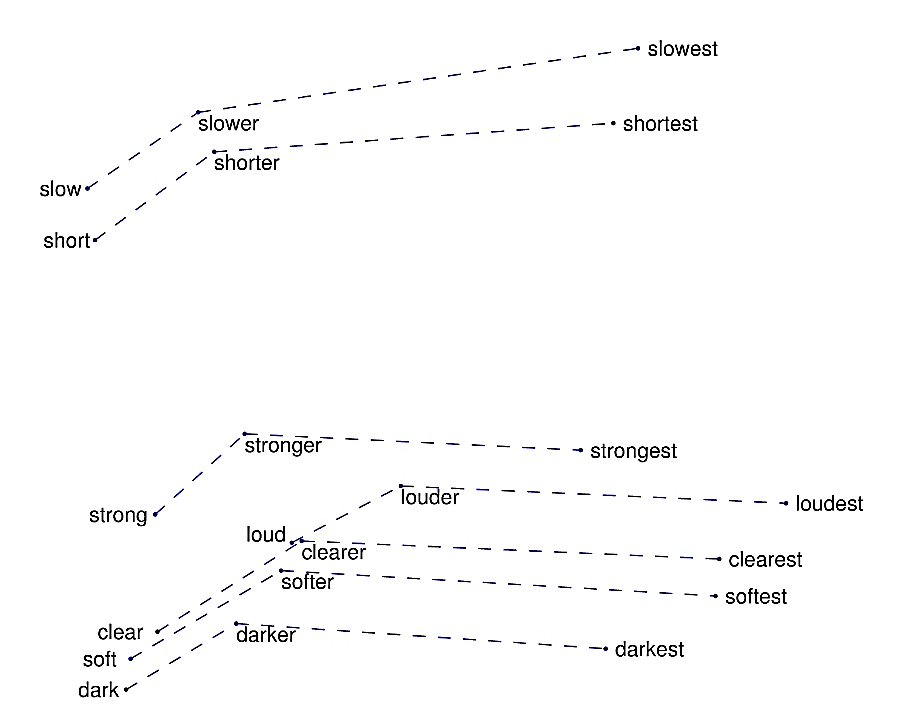
\includegraphics[width=0.65\textwidth]{comparativeVsSuperlative.png}}
\caption[t-SNE Visual of Comparative and Superlative Words]{
    t-SNE visual of GloVe word embeddings for select comparative and superlative words \cite{comparativeVsSuperlative}
}
\label{fig:comparativeVsSuperlative}
\end{figure}


The word embedding model used in this study is the GloVe model that was trained by a team of Stanford researchers using global word-to-word co-occurrence statistics.  This vector representation model proves to be highly effective at grouping together similar or related words in higher dimensions.  Furthermore, the model was designed in way such that vector differences between two words' word embeddings capture "the meaning specified by the juxtaposition of two words" \cite{glove}.  For example, the conceptual difference between "short", "shorter", and "shortest" is similar to the difference between "slow", "slower", and "slowest".  Using the underlying words' GloVe word embedding vectors, this conceptual difference is mirrored by vector differences in the t-SNE plot in Fig. \ref{fig:comparativeVsSuperlative}.


\section{Sentiment Analysis} \label{sentimentAnalysisSection}

One common text categorization task is sentiment analysis, which is the identification of sentiment-related features such as the author's positive or negative orientation towards the subject of the text.  Closely related is opinion mining which relates to the extraction and analysis of opinion about entities.  In most literature, and in this paper, the two terms are used interchangeably since the two tasks have become synonymous with each other \cite{sentimentApp}.  Texts such as movie, book, or product reviews, are clear examples of authors expressing their opinions, and sentiments, towards the product.  Similarly, editorials and political texts express the author's sentiment toward the political candidate or the political action that is the subject of the text \cite{nbSentiment}.

Sentiment analysis can be performed at varying granularities: document-level, sentence-level, and aspect-level.  As the terminology hints, document- and sentence-level sentiment analysis aim to classify the sentiment of the text using the whole document as a singular unit.  By classifying constituent sentences, a heuristic can be applied using these lower-level results.  On the other hand, aspect-level sentiment analysis aims to classify sentiment with respect to particular entities, such as parts of a products or distinct characteristics of a person \cite{sentimentApp}.

The potential, and observed, applications of sentiment analysis include product opinion gathering and monitoring, bias detection, automated recommendation engines, and even question answering and automated summarization \cite{sentimentAnalysis}.  Tasks such as product reception, review analysis, and suggesting other products to users based on their reviews are textbook examples of document- and sentence-level sentiment analysis.  Effective question answering systems need to be able to discern the aspect with which questions are asked; that is, whether not the question is purely fact-oriented, or is inherently opinionated and, thus, seeks an opinion-oriented response.  Similarly, summarization benefits from understanding the viewpoints of the text to provide a more cohesive output.


\section{$K$-Nearest Neighbors} \label{knnSection}

The $k$-nearest neighbors (KNN) algorithm is a decision-boundary based classification algorithm that classifies an input to the majority class of its $k$ nearest neighbors in space \cite{knnIR}.  The tunable hyperparameters for this algorithm include $k$, the number of neighbors used for classifying any given input, and the distance metric used for determining the closest neighbors.  The least robust KNN is thought to be $k$ = 1 because this model runs the risk of becoming heavily reliant on noise or outliers.  Variants of KNN may weigh the votes of training set observations with their cosine similarity relative to their input, as shown in Eq. \ref{eq:knnClassScore}.

\begin{equation}
\label{eq:knnClassScore}
score(c, d) = \sum_{d' \in S_{k}(d)} (I_{c}(d') \cdot cos(v(d'), v(d))
\end{equation}

In this scoring weighting scheme, $S_{k}(d)$ is the set of $d$'s $k$ nearest neighbors and $I_{c}(d')$ is the indicator function which equals 1 if and only if the observation $d'$ is part of class $c$, otherwise 0 \cite{knnIR}.

The advantages of KNN as a classification algorithm for practical applications are numerous.  As a non-parametric learning algorithm, KNN requires no assumption on the underlying distribution of the input data.  For applications in natural language processing, specifically classification of news articles as genuine or maliciously authored for political gain, there is not enough substantial evidence to map the articles' text to a closed form probabilistic distribution.  Furthermore, since KNN is an instance-based algorithm, the only "learning" required is to load the observations into memory, which significantly reduces training time \cite{knnGuide}.

As with any machine learning algorithm, KNN also has some drawbacks.  Testing inputs with KNN requires all of the training set to be in memory, or available through some highly performant data store, like a database, so vectorized inputs can be compared with every training point to determine the $k$ nearest neighbors.   However, because our dataset is not too large, this limitation is not a burden for our task.  Another downside to KNN is the time cost for testing: for each individual input, every training point must be checked to see if it is one of the $k$ nearest neighbors, and if so, use its label for classification.  As it turns out, even this limitation does not severely impact testing performance due to the size of the dataset; thus, a trained KNN model is highly performant and can be used for real-time classification \cite{knnGuide}.


\section{Support Vector Machines} \label{svmSection}

The support vector machine (SVM) classifier is a high performing machine learning algorithm that relies on the relatively simple concept of dividing the data into distinct regions.  For example, in binary classification, SVMs seek to maximize the distance between the data points of opposing classes and the dividing decision boundary.   The decision boundary, also known as the hyperplane, is formulated as a linear combination of weights on each dimension of the input, as shown in Eq. \ref{eq:hyperplane}.  $w$ is the vector of weights applied to input $x$, a support vector, whose length corresponds to the dimensionality of $x$, and $b$ is the bias, a constant offset.


\begin{equation}
\label{eq:hyperplane}
w^{T}x + b = 0
\end{equation}


The data points closest to the hyperplane are called the support vectors, and the shortest distance between these points and the boundary is called the margin.  By maximizing the margin, the probability for misclassification due to noise is reduced, assuming that the testing data points come from the same distribution as the training data.  One clear advantage of using SVMs is the low memory cost: only these support vectors need to be held in memory; the other data points, which are farther away from the hyperplane, no longer need to be considered (recall that the KNN algorithm requires every input be compared with every training observation to determine the most likely class) \cite{svmIR}.  

However, in most practical applications, the data cannot directly be separated into 2 well-defined regions, especially for complex datasets with a lot of overlap in the original feature space.  In these instances, it may be possible to map the feature space into a higher dimension where the classes are more easily separable.  However, this mapping may be too complex and computationally intensive to apply to large training sets \cite{svmTutorial}.  This computational complexity can be avoided altogether by using symmetric kernel functions on the pair of vectors, which results in a similarity score that is exactly equivalent to the dot product of its inputs when mapped into a higher dimensional space without having to explicitly map the vectors and computing their dot product, as shown in Eq. \ref{eq:kernelSubstitution} \cite{bishop}.


\begin{equation}
\label{eq:kernelSubstitution}
K(x, x') = \phi(x)^{T}*\phi(x') = \phi(x')^{T}*\phi(x) = K(x', x)
\end{equation}


One example use-case for this higher-order mapping is when the classes' data points are radially dependent.  As shown in Fig. \ref{fig:radialSeparation}, the data can be mapped to $R^{3}$ using the mapping function in Eq. \ref{eq:r3Mapping}.


\begin{equation}
\label{eq:r3Mapping}
z^{2} = x^{2} + y^{2}
\end{equation}


\begin{figure}[h]
\centering
\captionsetup{justification=centering,width=0.95\textwidth}
\centerline{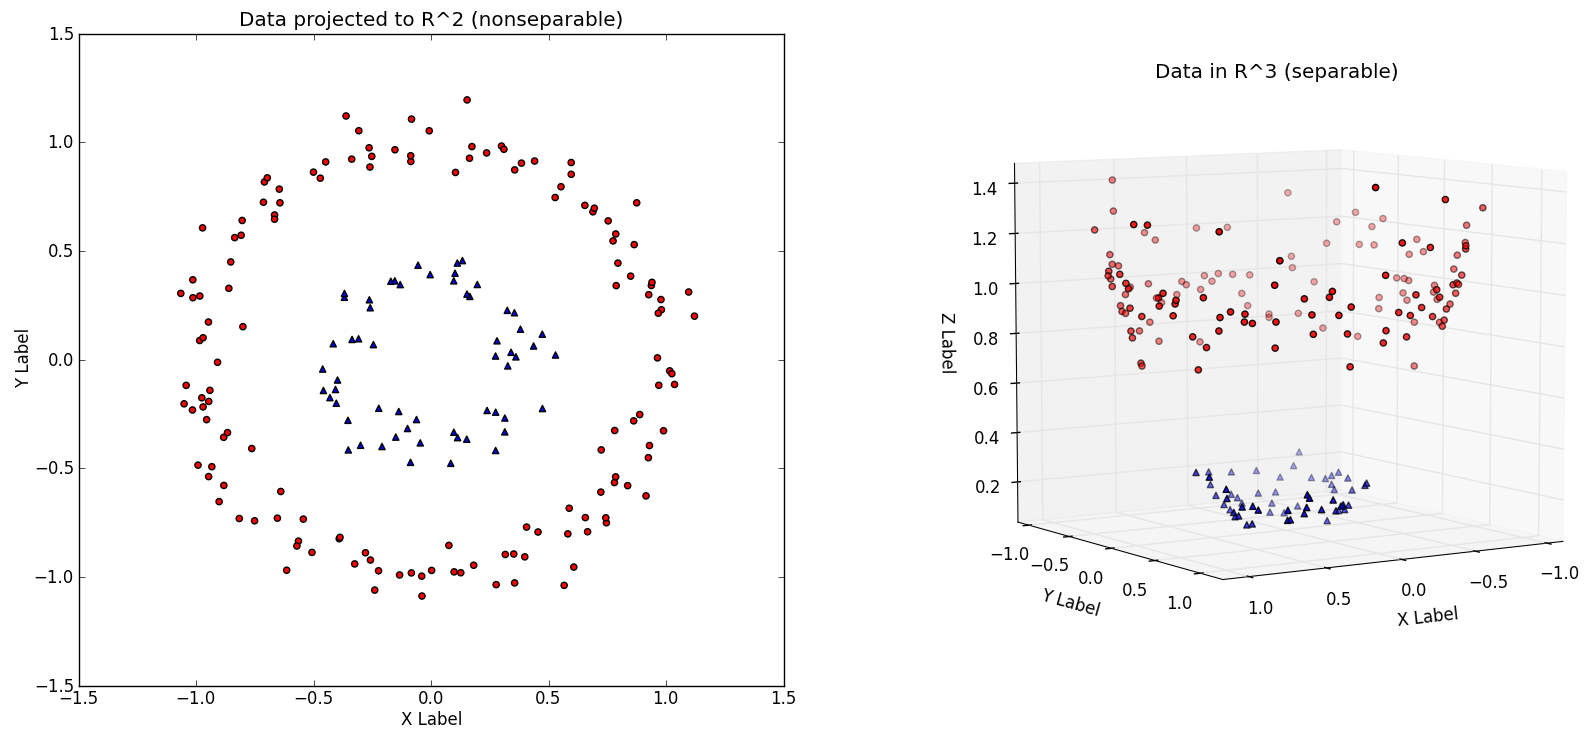
\includegraphics[width=0.95\textwidth]{radialSeparation.png}}
\caption[Mapping Observations from Radially Dependent Classes]{
    Visualizing 2-dimensional observations from two radially dependent distributions \cite{radialSeparation}\\
    Left: 2-D plot of the dataset where $x$ is the X-Label and $y$ is the Y-Label\\
    Right: Dataset is mapped into $R^{3}$ where $z$ is the radius from the origin
}
\label{fig:radialSeparation}
\end{figure}


The analogous radial basis function (RBF) kernel, also known as the Gaussian kernel, is show in Eq. \ref{eq:rbfEq} \cite{rbfKernel}:


\begin{equation} \label{eq:rbfEq}
K(x, x') = exp(-\gamma \cdot ||x-x'||^{2})
\end{equation}


\section{Neural Networks} \label{nnSection}

One of the most popular models that can be found in a modern-day machine learning engineer's toolkit is a neural network.  Though they are at the forefront of many modern  advances and innovations in artificial intelligence, they are far from new.  The idea of an artificial neuron dates as far back to 1943 when McCulloch and Pitts used their knowledge of neurology to devise their mathematical neuron that emulated simple neurons that acted in a binary fashion by firing when the sum of their inputs surpassed some internal threshold \cite{mccullochPitts}.  This simple neuron from 1943 is the foundation for the basic unit now known as a perceptron: a node with various inputs that are summed together to produce a binary result.  A perceptron (shown in Fig. \ref{fig:perceptron}) on its own is the simplest, single-layer neural network, and the weighted sum of its inputs models a linear classifier that can be used for binary classification.  In fact, the optimal values for each weight is learned during training just as the weights and bias are learned for a linear classifier.


\begin{figure}[h]
\centering
\captionsetup{justification=centering,width=0.95\textwidth}
\centerline{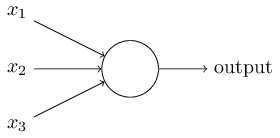
\includegraphics[width=0.65\textwidth]{perceptron.png}}
\caption[Perceptron Model] {
    A perceptron with three inputs: $x_{1}, x_{2}, x_{3}$ \cite{perceptron}
}
\label{fig:perceptron}
\end{figure}


Another key parameter when training a perceptron is its activation function, the input dependent function that decides whether or not the perceptron fires, that is, whether its output is 0 or 1.  In fact, if the simple perceptron emulates a linear classifier with the form in Eq. \ref{eq:hyperplane}, the perceptron's activation function is the Heaviside function (aka step function) since it classifies input vectors as class 0 on negative values and class 1 on positive values.  This classifier is also known as the simplest artificial neural network (ANN or NN) because it is a single layer of perceptrons: the weighted inputs are fed directly to the outputs.  To build more a complex model capable of making more complex decisions, layers of perceptrons are combined to create a network of nodes.  Such networks have historically been called multi-layer perceptrons (MLPs), even though modern networks are usually composed of neurons with other activation functions like the sigmoid, tanh, and rectified linear unit (ReLU) functions, which are shown in Fig. \ref{fig:activationFn} \cite{neuralNetsNLP}.


\begin{figure}[h]
\centering
\captionsetup{justification=centering,width=0.95\textwidth}
\centerline{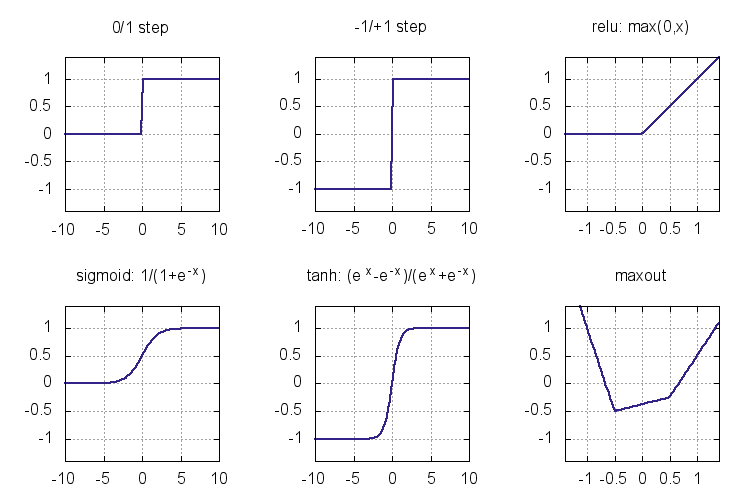
\includegraphics[width=0.95\textwidth]{activationFn.png}}
\caption[Activation Functions]{
    Common activation functions for artificial neurons \cite{activationFn}
}
\label{fig:activationFn}
\end{figure}


The layers that provide the interface between the input and output nodes are called hidden layers.  In typical feedforward networks, the layers of the network are fully connected, and unidirectional.  Thus, the information is strictly moving forward from the input towards the output and there are no cycles or loops.  Typical training of neural networks involves choosing the optimal architecture for the application, which in turn implies choosing the number of hidden layers, and number of nodes in each hidden layer.  The weights of the links between nodes are usually initialized to random values, and then trained with a technique called backpropagation.  Using the chosen loss function that penalizes misclassifications, the delta, or the difference between the model output and true value, of each training iteration is propagated backwards through the network to incrementally update the weights in order to minimize the loss function.  The learning rate of the model dictates at what pace the weights will follow the direction of the delta.  High learning rates will cause the model to take large steps in the direction of the delta, possibly overshooting the minimum and requiring extra iterations; on the other hand, smaller learning rates may lead to slower or incomplete training since many more iterations may be required to reach the minimum loss \cite{neuralNetsNLP}.


\section{Recurrent Neural Networks} \label{rnnSection}

Another class of neural networks showing great promise in the NLP domain is the recurrent network.  In contrast to feedforward networks, recurrent neural networks (RNNs) have directed cycles.  The primary advantage that cycles provide to RNNs is the ability to "[remember] information about what has been calculated so far" since each internal state is dependent on all of the previous computations and states leading up that state \cite{introRNN}.

The cycle in the RNN also allows the RNN to continuously transition between internal states for the entire length of the input sequence.  Thus, while basic feedforward neural networks have strict dimensional requirements for their input and output vectors, RNNs are able to dynamically operate on sequences of vectors \cite{rnn}.  For example, if the input sequence is a sentence with 5 words, the unrolled network would have 5 layers.  Fig. \ref{fig:rnnUnrolled} shows an RNN that unfolds into t+1 layers, where each layer (\textbf{A}) represents an internal state that was computed using the previous state and the next available piece of the input sequence (\textbf{x\textsubscript{t}}).  Note that an activation function can also be applied at each internal state to produce an output (\textbf{h\textsubscript{t}}).


\begin{figure}[h]
\centering
\captionsetup{justification=centering,width=0.95\textwidth}
\centerline{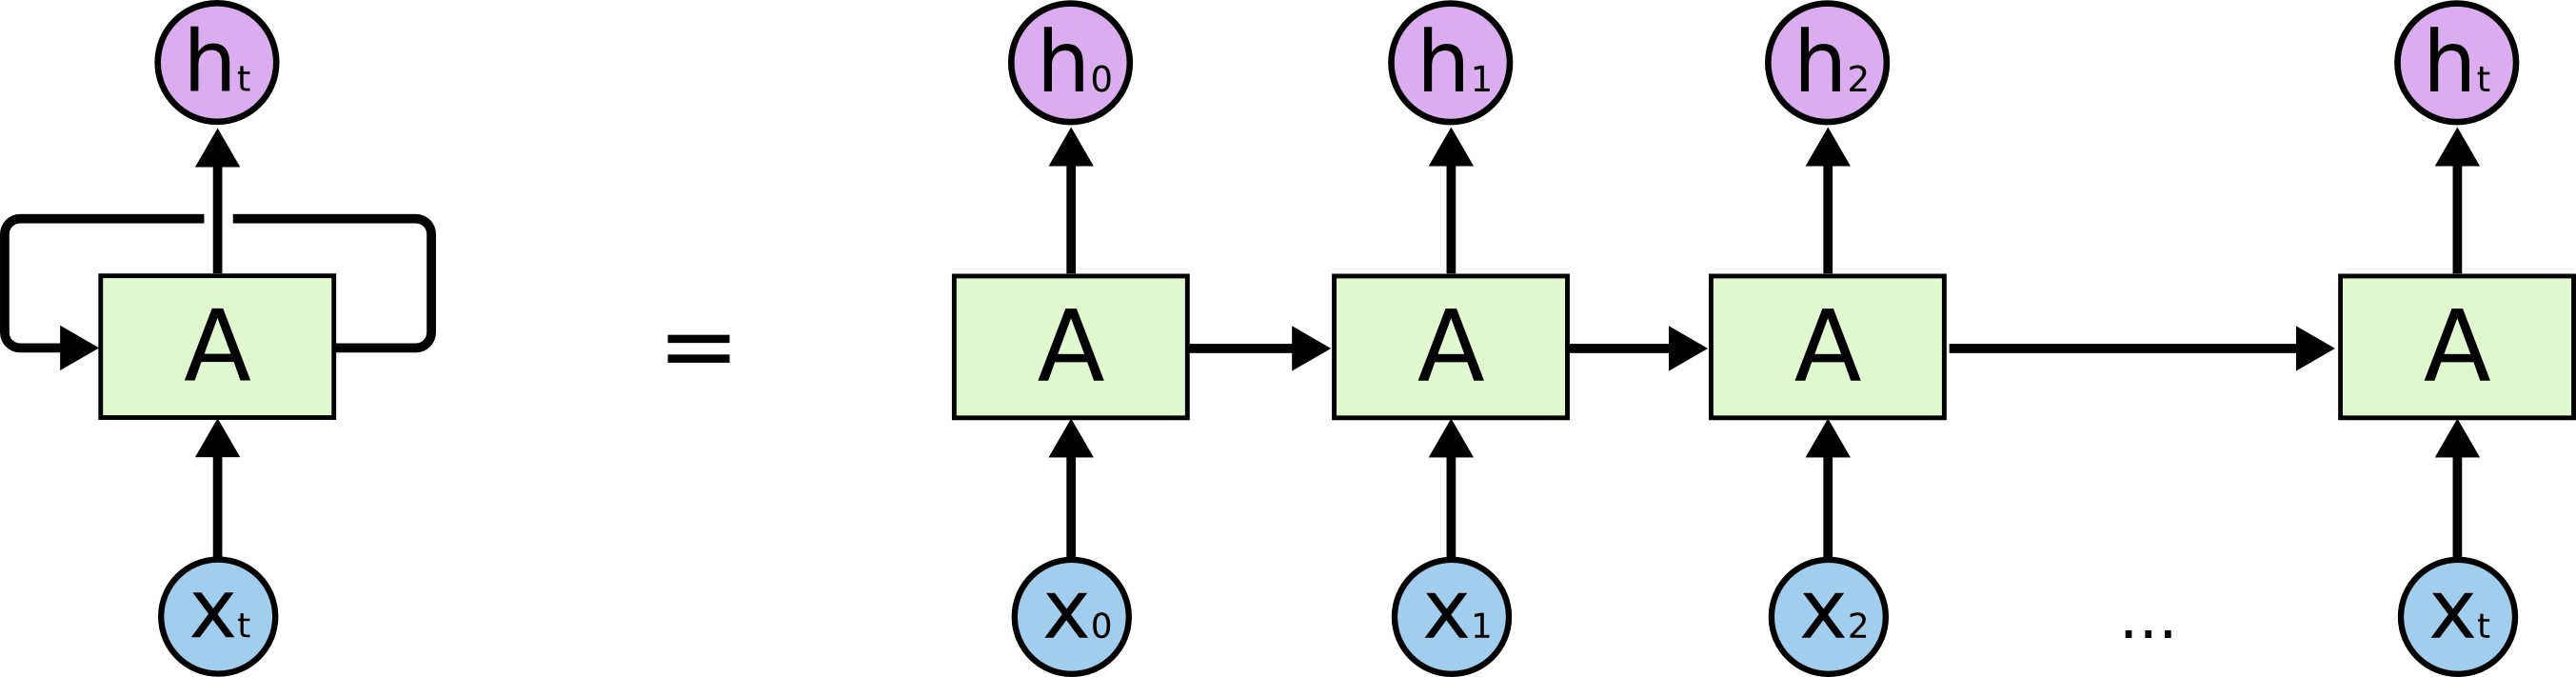
\includegraphics[width=0.95\textwidth]{rnnUnrolled.png}}
\caption[Unrolled RNN]{
    An RNN unrolled into a neural network with t+1 layers \cite{rnnUnrolled}
}
\label{fig:rnnUnrolled}
\end{figure}


Some applications for which RNNs have proven useful include speech transcription, machine translation (translating one language to another), video frame classification, and image captioning \cite{rnn}.  These applications all require the RNNs' stateful transitioning while processing the sequence of input; for example, producing a valid translation greatly depends on the part of sentence previously translated.  Furthermore, RNNs have also proven themselves to be highly performant in the absence of sequential input, as was the case in DeepMind's RNN that transcribed house numbers from Google Street View \cite{deepMindHouseNumber}.


\begin{figure}[h]
\centering
\captionsetup{justification=centering,width=0.95\textwidth}
\centerline{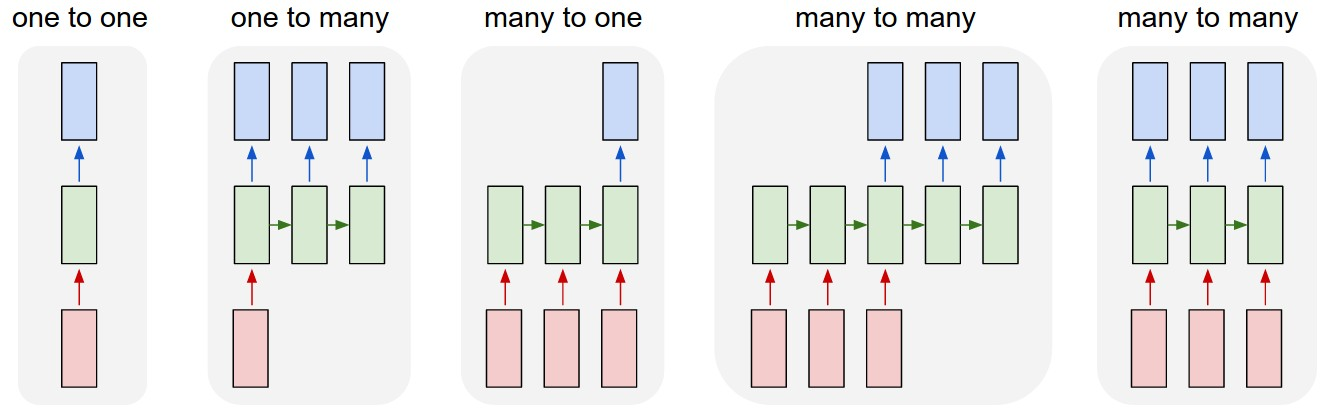
\includegraphics[width=0.95\textwidth]{rnnTransformations.png}}
\caption[Various RNN Setups]{
    The various use-cases for RNNs (green blocks) using input vectors (red) to produce output (blue) \cite{rnnTransformations}
}
\label{fig:rnnTransformations}
\end{figure}


As shown by Fig. \ref{fig:rnnTransformations}, RNNs can be used in a variety of settings.  The left-most setup ("one to one") demonstrates the transformation that occurs in typical neural networks: the input vector is processed completely by all of the hidden layers and then mapped to an output vector.  The "one to many" setup shows a transformation that may occur in settings like image captioning where a fix-sized image is transformed into a sequence of words.  The next setup, "many to one", illustrates how a sequential input is processed to produce a single label, which could be applied towards applications like sentiment classification.  The first "many to many" setup exemplifies the transformation that sentences could undergo in machine translation applications: input sequences are mapped to the target language using local context as opposed directly mapping each word independently.  Lastly, the second "many to many" configuration depicts a scenario in which an output is required for each constituent of the input sequence, e.g., a video classification task that requires labelling each frame \cite{rnnTransformations}.

However, there is a flaw with conventional RNNs.  The current state of an RNN, though dependent on previous parts of the input sequence, may be too far removed from the state at which a relevant piece of information was introduced.  For example, in the input sentence "I grew up in France... I speak fluent [language]", the RNN may not be able to predict "French" as the language since the word "France" occurred a lot earlier than where that information was actually necessary.  This gap between the necessary information and the point at which that information is actually needed may ultimately become too large for the RNN to be effective \cite{lstm}.  However, there is a special variant of the RNN, the long short-term memory (LSTM) network, that can overcome this limitation.

LSTMs are RNNs with special memory units (also known as cells) that can selectively keep information for an extended period of time \cite{lstmClassification}.  Instead of only consisting of a single repeating layer, as is the case with an RNN, the vanilla LSTM has one memory unit composed of four special layers: three sigmoid layers, and one tanh layer \cite{lstm}.  All sigmoid layers output values between 0 and 1, and the tanh layer outputs values between -1 and 1.  Together, these layers help the cell forget, remember, update, and produce information.

\begin{figure}[h]
\centering
\captionsetup{justification=centering,width=0.95\textwidth}
\centerline{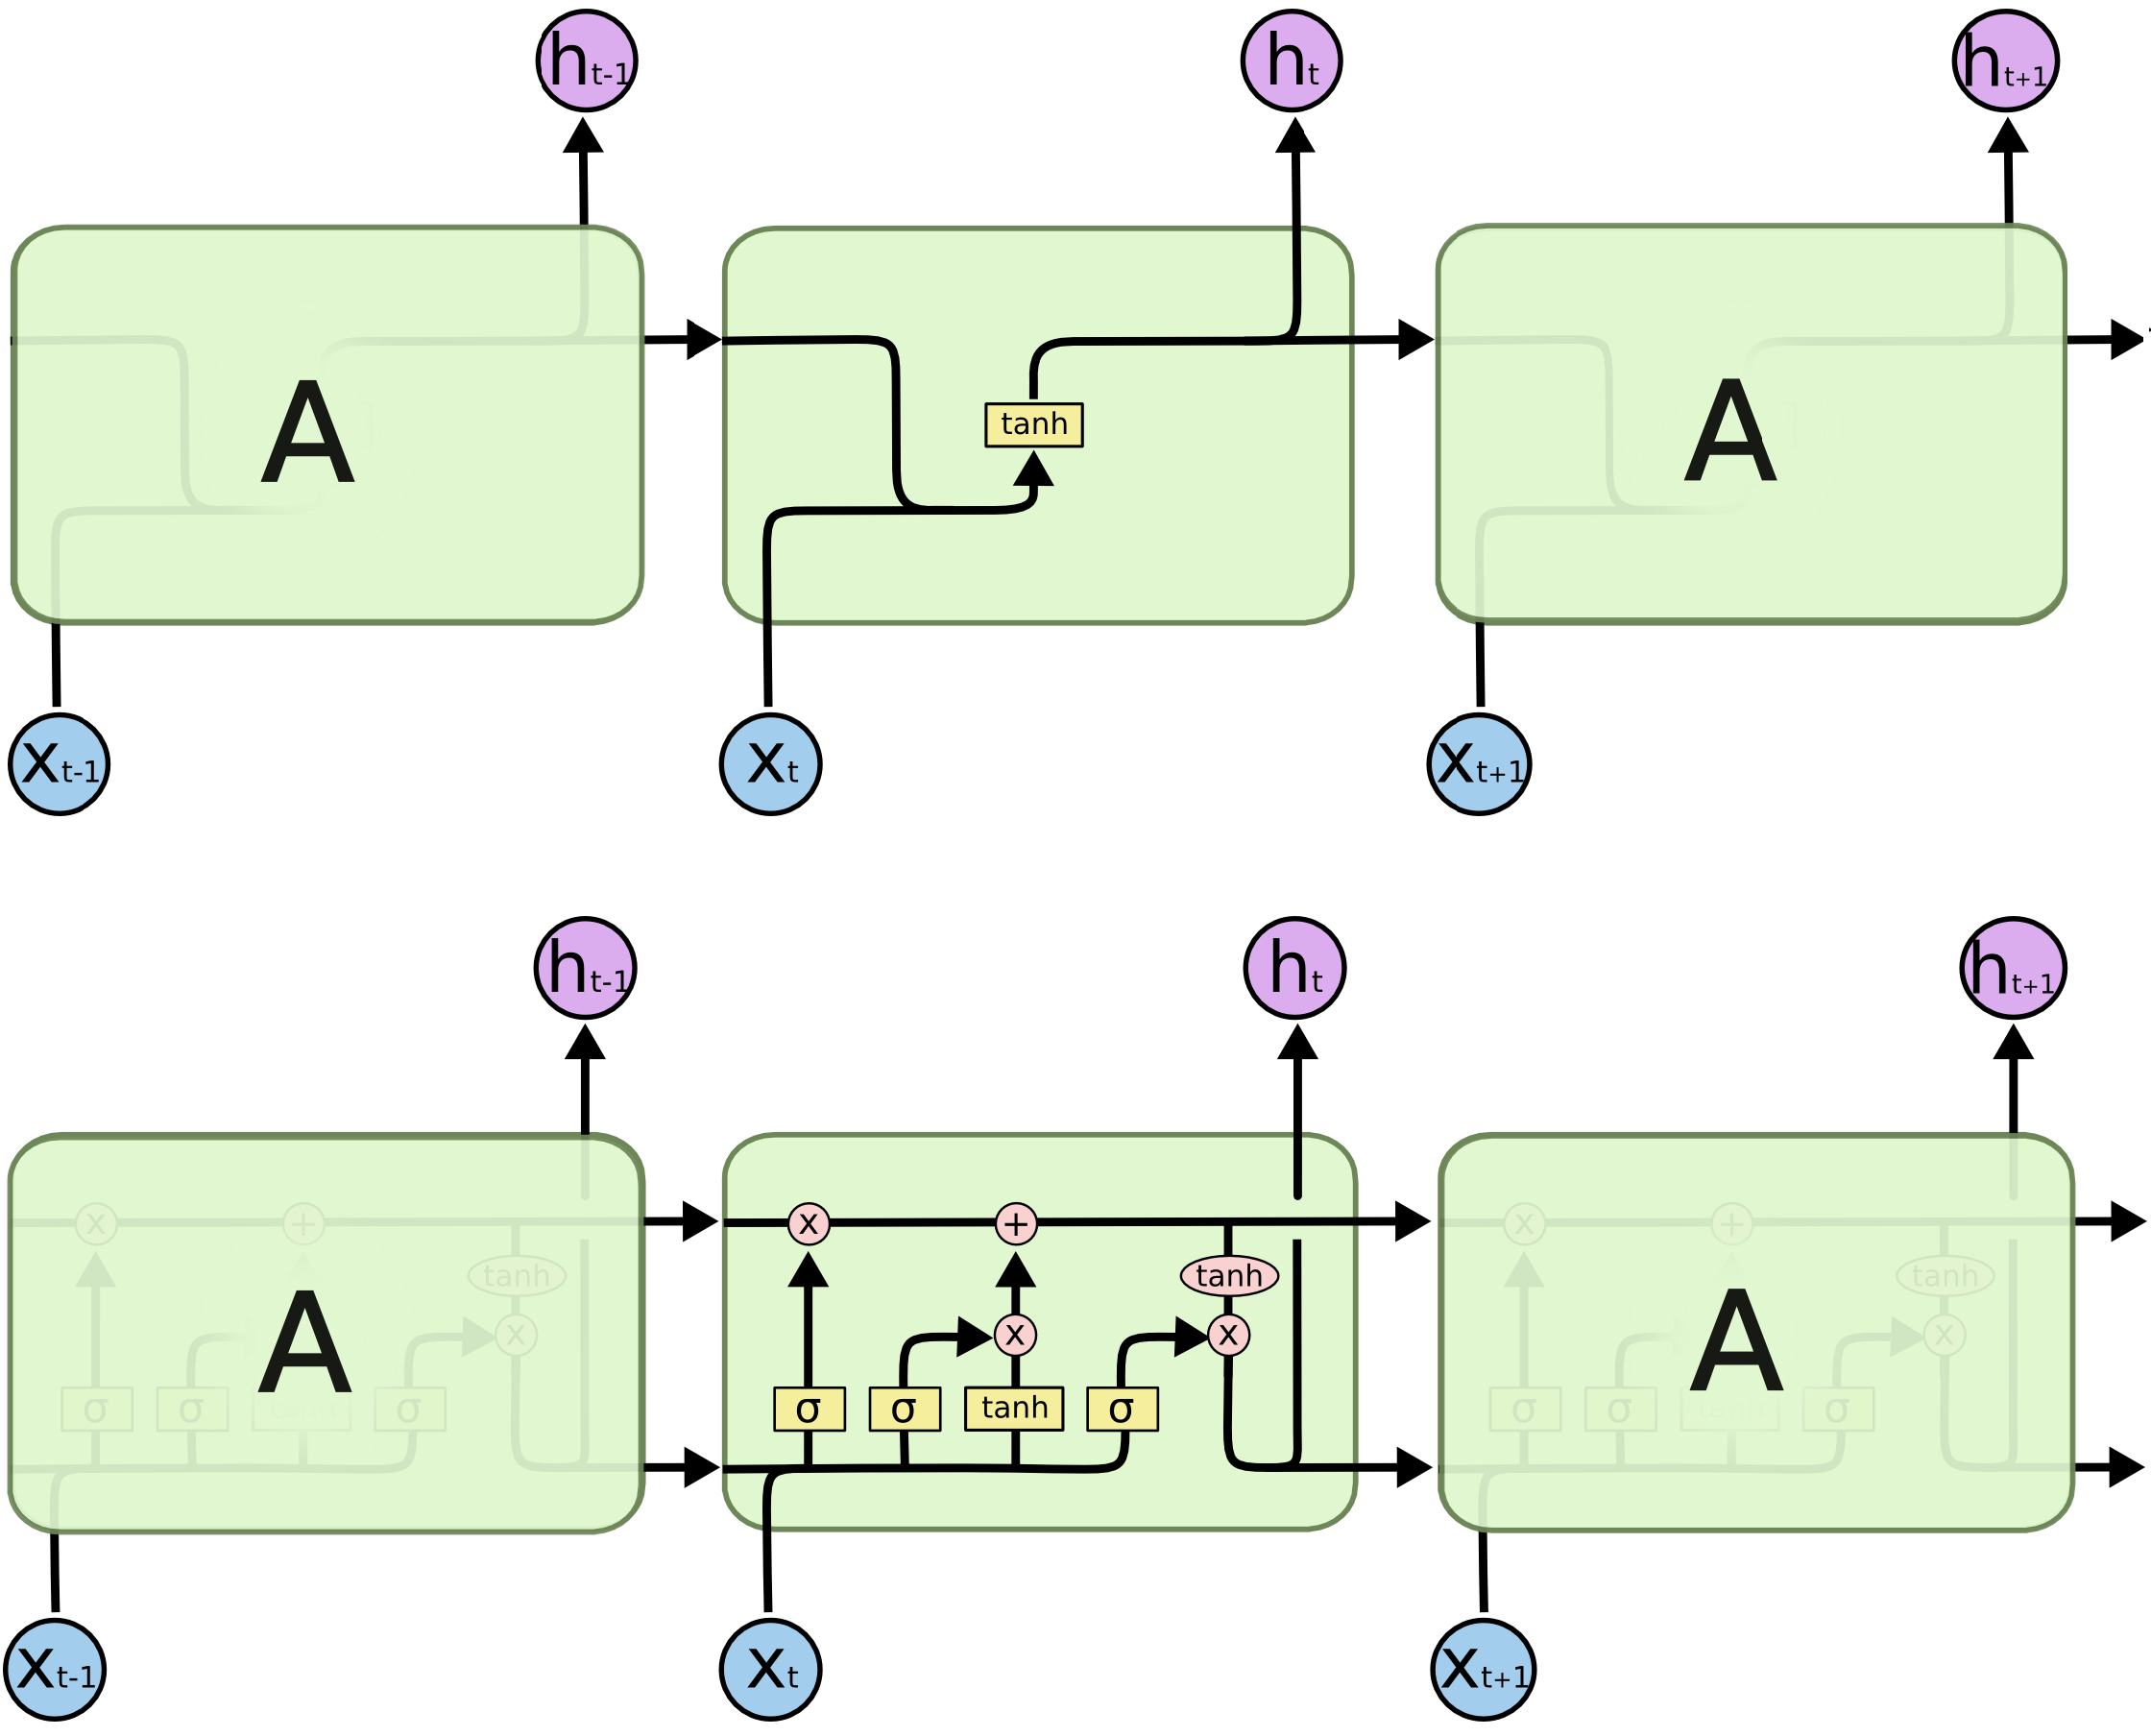
\includegraphics[width=0.95\textwidth]{rnnChainlstmChain.png}}
\caption[RNN Layer vs LSTM Layer]{
    Unrolled RNN and LSTM chains\\
    Top: RNN with a single layer in each state \cite{rnnChain}\\
    Bottom: LSTM with one memory unit in each state \cite{lstmChain}
}
\label{fig:lstmChain}
\end{figure}

As shown in the LSTM in Fig. \ref{fig:lstmChain}, the first layer is a sigmoid layer whose input is the concatenation of the output from the previous state (\textbf{h\textsubscript{t-1}}) and the current input (\textbf{x\textsubscript{t}}).  In LSTMs, sigmoid layers that are joined with pointwise multiplication operators act as gates that let information through whenever their outputs are non-zero values.  The first sigmoid layer uses \textbf{h\textsubscript{t-1}} and \textbf{x\textsubscript{t}} and forms a gate on the incoming stream of values from the previous cell state (the top left corner of each cell in Fig. \ref{fig:lstmChain}).  This gate, often called the "forget gate", outputs a number between 0 and 1 for each value in the previous state.  Thus, if the gate outputs 0 for a particular value, that value is completely forgotten.

The next stage of the cell decides how much of the new information (\textbf{h\textsubscript{t-1}} and \textbf{x\textsubscript{t}}) will be retained in the state.  First, a tanh layer is used to compute an updated value for each bit of new information.  Afterwards, these updated values are filtered by another gate in order to extract whatever is deemed pertinent by the LSTM.  Finally, the filtered information is added with whatever information from the previous state that was not forgotten to form the new cell state.

The last stage of the cell computes the output for the current state (\textbf{h\textsubscript{t}}).  The first step in this stage is to map the cell state into the acceptable output space.  In Fig. \ref{fig:lstmChain}, the tanh activation function is applied to the cell state to push each value between -1 and 1.  The transformed state is then passed through the final sigmoid gate; thus, the output consists of only the parts of the cell state the LSTM deems appropriate.  For example, in a machine translation setting, the LSTM may output whether or not the subject is singular or plural, so the LSTM knows how to conjugate the following verb if that is in fact the following input \cite{lstm}.

There are other LSTM configurations, and each has its own advantages in certain settings.  However, a recent study shows that most of these variations do not perform significantly better than the vanilla LSTM \cite{variousLSTMs}.  The LSTM model used in this thesis is a variant of the vanilla LSTM model that has a configurable number of memory units \cite{kerasLSTM}.  Note that the LSTM presented in this section only had a single memory unit, and, thus, produced a single output.  Adding extra memory units increases the dimensionality of the output at each state.  Thus, if the LSTM contains 50 memory units in each layer, the LSTM will ultimately produce a 50-dimensional output vector after processing the entire input sequence.  Since the challenge presented in this thesis is a binary classification task, the outputs of each LSTM are passed through another sigmoid activation layer to produce a prediction.
